% vim: set spelllang=fr foldmethod=marker:
\chapter{Introduction}\label{chap:in}

% préfixe: in
\renewcommand\chapterpath{Main/Intro}
\renewcommand\chapterfig{Main/Intro/Figures}

\vfill
\begin{figure*}[!ht]
    \centering
    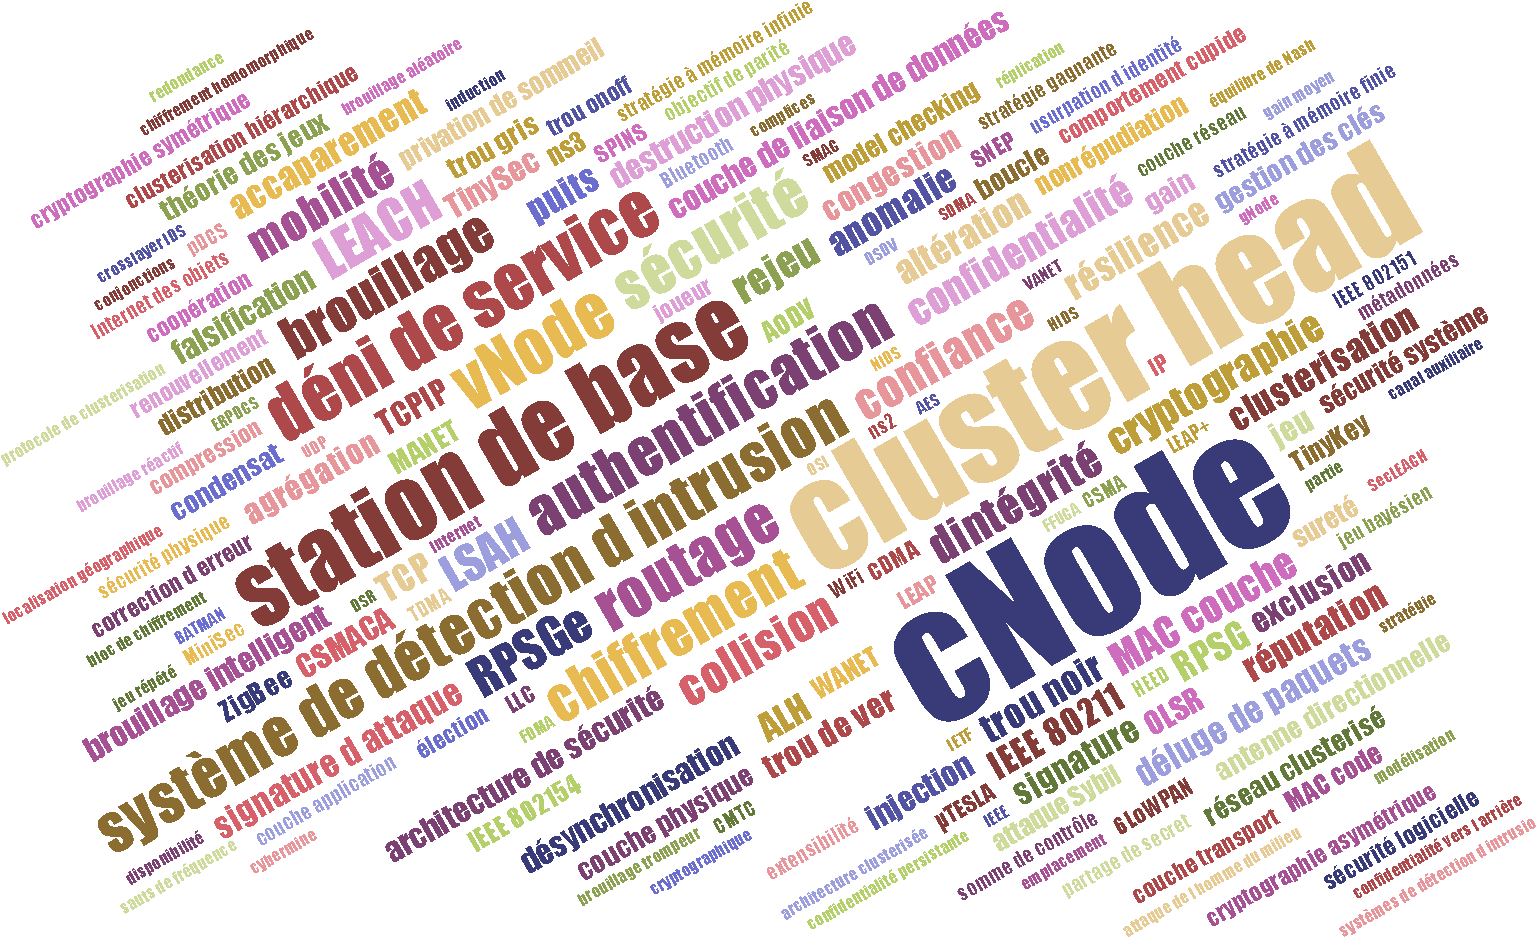
\includegraphics[width=\textwidth]{\chapterfig/cloud30v1.pdf}
    \caption[Nuage des mots-clés indexés de l'ouvrage]{Nuage des mots-clés indexés de l'ouvrage. L'échelle des mots est relative à la racine carrée du nombre d'occurrences.}
\end{figure*}
\vfill
\pagebreak
% vim: set spelllang=fr foldmethod=marker:
\section{Réseaux de capteurs sans fil et déni de service}

\lettrineh{L}{a lutte} contre les attaques de type «déni de service» dans les réseaux de capteurs sans fil est le fil directeur des travaux présentés dans cet ouvrage.\linebreak
Les réseaux de capteurs sont constitués de petits appareils ---~les capteurs~--- équipés d'un module de communication sans fil.
Dispersés dans l'environnement à étudier, ces capteurs sont chargés de réaliser des mesures physiques, de les convertir en un signal numérique, et de les rapatrier pour un traitement plus approfondi à une station de base, qui fait office d'interface entre le réseau et l'utilisateur.
Cette collecte d'information est soumises aux contraintes en ressources des capteurs, dont les capacités en calcul, en mémoire, et dont la réserve d'énergie disponible en batterie sont limitées.

Mais les protocoles déployés ont su être adaptés: les capteurs sont aujourd'hui utilisés dans une multitude d'applications dans des domaines aussi variés que l'environnement, la santé, l'urbanisme, les transports, la domotique, et bien sûr le domaine militaire.
Liés à la fois aux avancées technologiques et à l'émergence de nouveaux usages dans l'exploitation des données, les concepts de «transports intelligents», de «villes intelligentes» ou d'«Internet des objets» se développent peu à peu et semblent promettre un usage de plus en plus intensif des réseaux de capteurs sans fil.

Toutefois, ces réseaux particuliers introduisent leur lot de problématiques: à côté des contraintes fortes en ressources se pose la question de la sécurité, dont la mise en place est une nécessité absolue pour les applications médicales ou militaires par exemple.
Alors que les mécanismes d'authentification et de chiffrement font appel, dans la plupart des systèmes informatiques, à des protocoles cryptographiques couteux en ressources, il a fallu adapter les mécanismes au monde des capteurs.
Mais la sécurité comporte d'autres volets, et la disponibilité des réseaux, suivant le contexte, peut s'avérer tout aussi essentielle.

En résumé, le problème se pose ainsi: comment prévenir, ou à défaut comment détecter puis contourner, tout en économisant les ressources des capteurs, une action d'origine malveillante qui viserait à mettre le réseau hors service?
Cette thèse s'appuie sur l'attribution d'un rôle de surveillance à certains des capteurs, chargés de détecter des comportements hostiles au sein du réseau, et de prévenir leurs pairs lorsqu'une attaque est détectée.

C'est notamment le processus de sélection dynamique de ces capteurs de surveillance qui fait l'objet d'une étude poussée.
Plusieurs solutions sont proposées: une sélection aléatoire, permettant d'obtenir statistiquement une bonne couverture du réseau; une sélection basée sur l'énergie résiduelle des capteurs, dont l'avantage est d'offrir une meilleure répartition de la charge (en termes de consommation énergétique) dans le réseau; et enfin un processus d'élection démocratique, basé sur des scores de réputation, qui améliore encore la sécurité du dispositif.

Mais en sus des algorithmes concrets, il est parfois utile de pouvoir représenter un processus sous un aspect plus formel.
Validées par des simulations, certaines des méthodes proposées sont également modélisées à l'aide de chaines de \textsc{Markov} ou de réseaux de \textsc{Petri} particuliers.
En fin d'étude, les jeux quantitatifs sont utilisés pour caractériser à plus haut niveau le système comportant un capteur corrompu et des capteurs de surveillance.
\pagebreak %%%%%%%%%%%%%%%%%%%%%%%%%%%%%%%%%%%%%%%%%%%%%%%%%%%%%%%%%%%%%%%%%%%%

Le but des travaux présentés dans cette thèse est donc de proposer, dans un temps, un ensemble de méthodes de détection et de réaction efficace aux attaques de déni de service, tout en économisant ou en répartissant au mieux la consommation énergétique des capteurs pour prolonger le plus possible la durée de fonctionnement du réseau.
Les outils de modélisation fournis permettent à la fois de valider ces méthodes, de mieux les comprendre, et avec un peu de chance, de servir de base dans le futur pour la conception de mécanismes toujours plus performants.

% vim: set spelllang=fr foldmethod=marker:
\section{Organisation de la thèse}

